\section{Métodos computacionales}

\subsection{Método DFTB}\label{s:dftb}

El formalismo del funcional de densidad de enlace estrecho (DFTB, \textit{density
functional tight-binging}) que se utiliza los capítulos \ref{ch:modelo} y 
\ref{ch:prediccion} ha sido ampliamente descripto en la literatura 
\cite{elstner1998,frauenheim2000,seifert2007,gaus2011}. El método DFTB se basa 
en una expansión a segundo orden de la energía de la teoría del funcional de la 
densidad (DFT) con respecto a una fluctuación de la densidad electrónica de 
referencia \cite{foulkes1989}. La energía de DFTB resultante puede escribirse de 
la siguiente manera:
\begin{equation}\label{eq:dftb}
    E_{\text{DFTB}}=\sum_i^{\text{occ}}\langle\Psi_i|\hat{H}^0|\Psi_i\rangle+\frac{1}{2}\sum_{AB}\gamma_{AB}\Delta q_A\Delta q_B+E_{\text{rep}}^{AB}
\end{equation}
donde $\Psi_i$ denota los orbitales Kohn-Sham (KS) de una partícula. Con una 
combinación lineal de orbitales atómicos, $\Psi_i$ se expande en un conjunto de 
orbitales de valencia pseudoatómicos de tipo Slater $\phi_\nu$,
\begin{equation}
    \Psi_i({\bf r})=\sum_\nu c_{\nu i}\phi_\nu({\bf r}-{\bf r}_A),
\end{equation}
que se determinan resolviendo la ecuación secular KS
\begin{equation}\label{eq:ks}
    \sum_\mu c_{\mu i}\left(H^0_{\nu\mu}-\epsilon_iS_{\nu\mu}\right)=0, \;\;\forall \nu,i
\end{equation}
donde $S_{\nu\mu}=\langle \phi_\nu| \phi_\mu\rangle$ y $\epsilon_\nu$ son la 
matriz de superposición y los autovalores de un átomo aislado, respectivamente.
${H}^0_{\nu\mu}$ es el Hamiltoniano efectivo KS generado con la densidad 
electrónica de referencia, $\rho^0$, y está definido como
\begin{equation}\label{eq:h0}
    H^0_{\nu\mu}=\begin{cases}
        \epsilon_\mu & \text{si}\; \nu=\mu\\
        \langle \phi_{\nu}| -\frac{1}{2}\nabla^2+v_{\text{eff}}\left[\rho_A^0+\rho_B^0\right]|\phi_{\nu}\rangle&\text{si}\;\mu\in A,\; \nu\in B\;\text{y} \;A\ne B\\
        0& \text{si no}
    \end{cases}
\end{equation}
donde $\rho_A^0$ es la densidad de referencia de un átomo neutro $A$ y 
$v_{\text{eff}}$ el potencial KS efectivo, construido a partir de la superposición
de densidades centradas en átomos neutros. En particular, los elementos de la 
matriz del Hamiltoniano dependen solo de los átomos $A$ y $B$, por lo tanto sólo
se calculan explícitamente los elementos de dos centros de las matrices del 
Hamiltoniano y de superposición en función de la distancia y la orientación, usando 
las reglas de transformación de Slater-Koster \cite{slater1954}.

Una de las partes cruciales del uso del método DFTB es calcular las funciones de 
base y las densidades atómicas $\phi$ y $\rho^0$, respectivamente. Los orbitales
pseudoatómicos y las densidades se obtienen de resolver las ecuaciones atómicas KS 
modificadas en las que se agrega un potencial de confinamiento, $V_{\text{conf}}$
\begin{equation}\label{eq:dft}
    \left[\hat{T}+V_{\text{eff}}+V_{\text{conf}}\right]\phi_\mu=\epsilon_\mu\phi_\mu.
\end{equation}
Una práctica común dentro de la comunidad de DFTB consiste en elegir un potencial
de confinamiento parabólico o cuadrático. En esta tesis se utilizó una función 
de ley de potencia, como está implementada en el código \path{Hotcent}
\cite{hotcent, van2019},
\begin{equation}\label{eq:vconf}
    V_{\text{conf}}(r)=\left(\frac{r}{r_0}\right)^{\sigma}
\end{equation}
donde $r_0$ y $\sigma$ son números reales que pueden ser elegidos de para cada 
orbital atómico $\phi$ y cada densidad $\rho^0$.

\begin{table}[h!]
    \centering
    \caption{Configuraciones electrónicas, energías en el sitio de los orbitales
    de valencia y parámetros de Hubbard calculados con el funcional de intercambio
    y correlación PBE.}
    \setlength\extrarowheight{2pt}\stackon{%
    \begin{tabular}{l c c c c c}
        \toprule
        \textbf{Elemento} & 
        \textbf{Capa de valencia} &  
        \textbf{$\varepsilon_s$} &
        \textbf{$\varepsilon_p$} &  
        \textbf{$U_s$} & 
        \textbf{$U_p$} \\
        \midrule
        Li & 2s$^1$ & -0.105127 & -- & 0.167057 & -- \\
        Li & 3s$^2$3p$^2$ & -0.395452 & -0.150169 & 0.329247 & 0.244483 \\
        \bottomrule
    \end{tabular}
    }{}
    \label{t:hubbard}
\end{table}
El segundo término en la ecuación \ref{eq:dftb} es la energía debida a las 
fluctuaciones de cargas y se parametriza analíticamente como una función de las
cargas orbitales y de $\gamma_{AB}$, que a su vez es una función de la separación 
interatómica y del parámetro de Hubbard, $U$, (ver Tabla \ref{t:hubbard}) que se 
obtienen suponiendo que son iguales a los de los átomos aislados y se calculan
como la diferencia de la afinidad electrónica y la energía de ionización para 
distintos momentos angulares orbitales \cite{elstner1998b}. 
$\Delta q_X = q_X - q_X^0$ es la carga de Mulliken inducida autoconsistente en el 
átomo $X$ \cite{elstner1998}.

La contribución restante a la energía total de DFTB en la ecuación \ref{eq:dftb}
es $E_{\text{rep}}$ y se corresponde con el potencial repulsivo diatómico que 
depende de la distancia y contiene los efectos de los electrones del núcleo, los 
términos de repulsión ion-ion y efectos de intercambio-correlación. 
La energía total repulsiva de un sistema es una suma de contribuciones de 
potenciales repulsivos $V_{\text{rep}}(r)$ de cada par de átomos
\begin{equation}\label{eq:rep}
    E_{\text{rep}}=\sum_{i<j} V_{\text{rep}}(r_{ij})
\end{equation}
donde $i$ y $j$ son los índices de los átomos en el sistema y $r_{ij}$ es la 
distancia entre ellos. Generalmente se considera que $V_{\text{rep}}$ es una
función empírica que se determina de ajustar datos de cálculos de estructura 
electrónica de un nivel mayor, como DFT. En este capítulo, ajustó dicho potencial 
utilizando el código \path{TANGO} \cite{tango}, donde el potencial repulsivo 
viene dado por:
\begin{equation}\label{eq:v_rep}
    V_{\text{rep}}(r) = \begin{cases}
        e^{-a_1r+a_2}+a_3 & 0\le r<r_{\min}\\
        \displaystyle\sum_{i=2}^m c_i\left(r_{\text{cut}}-r\right)^i & r_{\min}\le r < r_{\text{cut}}\\
        0 & r_{\text{cut}} \le r
    \end{cases}
\end{equation}
los valores que se utilizan para $r_{\min}$ y $r_{\text{cut}}$ se encuentran
en la Tabla \ref{t:mincut}. Los parámetros $a_i$ se ajustan para reproducir las 
energías de DFT para cada estructura elegida para el entrenamiento utilizando el 
algoritmo de Levenber-Marquardt. Para el grado $m$ del polinomio se eligió 8 y 
los coeficiente $c_i$ se optimizaron con un ajuste por cuadrados mínimos.
Los códigos \path{Hotcent} y \path{TANGO} proveen valores por defecto para 
cualquier otro parámetro que no haya sido explícitamente descripto. 
\begin{table}[h!]
    \centering
    \caption{Valores de $r_{\min}$ y $r_{\text{cut}}$ utilizados en la ecuación
    \ref{eq:v_rep}}
    \setlength\extrarowheight{2pt}\stackon{%
    \begin{tabular}{l c c}
        \toprule
        & 
        \textbf{$r_{\min}$ [\AA]} & 
        \textbf{$r_{\text{cut}}$ [\AA]} \\
        \midrule
        Si-Si & 1.7760 & 3.4410 \\
        Si-Li & 1.7925 & 4.1825 \\
        Li-Li & 1.9456 & 4.7360 \\
        \bottomrule
    \end{tabular}
    }{}
    \label{t:mincut}
\end{table}


\subsection{Cálculos DFT}

Los cálculos de DFT de las estructures cristalinas fueron obtenidos usando el 
paquete de simulación \path{GPAW} ~\cite{enkovaara2010, mortensen2005} del 
Entorno de Simulación Atómica \cite{larsen2017}. El paquete \path{GPAW} es un 
algoritmo de grilla del espacio real basado en el método de la función de onda 
aumentada por proyector \cite{blochl1994} que utiliza la aproximación del núcleo 
congelado. Las coordenadas de Li, Li$_{15}$Si$_{4}$, Li$_{13}$Si$_{4}$, 
Li$_{7}$Si$_{3}$, Li$_{12}$Si$_{7}$, LiSi y Si se descargaron del Materials 
Project \cite{materials_project} (códigos mp: 135, 569849, 672287, 1201871, 1314, 
795 y 149) correspondiente al Li BCC, x $\approx$ 3.75, 3.25, 2.33, 1.71, 1 y
Si diamante, respectivamente. Los cálculos DFT se realizaron utilizando el 
funcional de intercambio-correlación PBE (Perdew-Burke-Ernzerhof) y la integración
de la zona de Brillouin se efectuó con grillas Monkhorst-Pack con una densidad
de 2.5 puntos $k$ por \AA$^{-1}$.

También se estudiaron con cálculos DFT estructuras amorfas de Li$_x$Si siguiendo
el protocolo de litiación propuesto por Chevrier y Dahn \cite{chevrier2009, 
chevrier2010}. Se utilizó un esquema de celda repetido con 12 átomos de silicio y 
$N$ de litio por celda unidad, con $N\in[0,45]$ cubriendo todo el intervalo 
$x\in[0,3.75]$. Cada estructura Li$_{N+1}$Si$_{12}$ se obtuvo agregando un átomo 
de litio en la esfera vacía más grande de la celda Li$_{N}$Si$_{12}$ y realizando
una optimización geométrica de las posiciones atómicas y del volumen de la celda.
En este caso, se realizaron los cálculos con el programa \path{QUANTUM} 
\path{ESPRESSO} \cite{quantum_espresso,quantum_espresso_advanced}, utilizando el 
funcional de intercambio-correlación PBE con una energía cinética de corte de 
1090 eV y una integración de la zona de Brillouin con grillas Monkhorst-Pack con 
una densidad de 7 puntos $k$ por \AA$^{-1}$. Las posiciones atómicas y el volumen 
de la celda se optimizaron utilizando el algoritmo BFGS hasta que la fuerza fuera 
menor a 0.08 eV/\AA\ para cada estructura.


\subsection{Algoritmo de ajuste}\label{s:algfit}

En esta tesis, todos los cálculos de DFTB fueron realizados con \path{DFTB+} 
\cite{dftb+}. Para la obtención de los parámetros Li-Si de DFTB se siguió el 
método de aprendizaje descripto en los trabajos de van den Bossche \textit{et al.}
\cite{van2018, van2019}. Esto se realizó para dos conjuntos de parámetros, 
denotados como conjunto A y conjunto B, que difieren entre ellos en el ajuste
del término de la energía de bandas. En el conjunto A se ajusta la estructura 
de bandas de Li y Si por separado, mientras que en el conjunto B se utiliza para 
esto la estructura Li$_7$Si$_3$. La elección de esta última estructura se debe a
que el valor para la energía de formación es el menor entre todas las aleaciones
cristalinas consideradas \cite{materials_project}. La parametrización de los 
orbitales pseudoatómicos y de las densidades electrónicas consisten en optimizar 
los valores de $r_0$ y $\sigma$ en la ecuación \ref{eq:vconf} para ajustar la 
estructura de bandas de referencia de DFT. La Tabla \ref{t:vconf_params} muestra
los valores de los parámetros de confinamiento optimizados.
\begin{table}[h]
    \centering
    \caption{Parámetros del potencial de confinamiento $r_0$ y $\sigma$ para 
    los orbitales atómicos $\phi$ y las densidades $\rho^0$ de Li y Si}
    \setlength\extrarowheight{2pt}\stackon{%
    \begin{tabular}{l ccccc ccccc}
        \toprule
        &\multicolumn{5}{c}{\textbf{conjunto A}}&\multicolumn{5}{c}{\textbf{conjunto B}}\\
            \textbf{Elemento} & \textbf{$r_0(\phi)$} & \textbf{$\sigma(\phi)$} & \textbf{$r_0(\rho^0)$} & \textbf{$\sigma(\rho^0)$} & & & \textbf{$r_0(\phi)$} & \textbf{$\sigma(\phi)$} & \textbf{$r_0(\rho^0)$} & \textbf{$\sigma(\rho^0)$}\\
        \midrule
         Li & $4.899$ & $1.889$ & $7.233$ & $1.986$ & & & $4.843$ & $1.927$& $7.210$ & $1.999$\\
         Si & $4.558$ & $6.909$ & $6.318$ & $2.188$ & & & $3.556$ & $2.382$& $6.292$ & $1.891$\\
        \bottomrule
    \end{tabular}
    }{}
    \label{t:vconf_params}
\end{table}

Por otro lado, el conjunto de datos de entrenamiento requerido para ajustar el 
término de repulsión de pares se obtuvo utilizando las estructuras cristalinas 
ya mencionadas. Llámese $S$ al conjunto de estructuras cristalinas. A cada una de 
ellas se le realizaron compresiones y expansiones isotrópicas utilizando un 
factor de escaleo que varió de 0.4 a 1.45 con un equiespaciado de 0.05 unidades, 
generando así 22 estructuras por estequiometría. La energía de cada estructura se 
computó con DFT y se descartaron aquellas que superaban los 10 eV del mínimo de 
la estequiometría. De este procedimiento se obtuvieron 108 estructuras para el 
conjunto de entrenamiento. Para cada estructura $s$ de una dada estequiometría 
en $S$ ($s \in S$) se denota por $N_s$ la cantidad de estructuras asociadas a 
ella. Además, para cada estequiometría $s$, se denota con ${\bf r}^s_i$ la 
$i$-esima estructura y con $\check{{\bf r}}^s$ la estructura correspondiente a la
menor energía de DFT. Se usará el símbolo ``$\ \check{\ }\ $'' para denotar 
el argumento del mínimo de otras funciones.

Teniendo esto en cuenta, se obtiene el conjunto de parámetros 
$\check{\bf p} = \left( \left\{\check{c}_i\right\}, \left\{\check{a}_i\right\}\right)$ 
(ver ecuación \ref{eq:rep}) de DFTB que minimizan la sumatoria de los residuos 
de la energía
\begin{equation}\label{eq:e_res}
    \text{Res}_E({\bf p})=\sum_{s\in S}\sum_{i=1}^{N_s} \omega^s_i
    \left[E_{\text{DFT}}({\bf r}^s_i)-(E_{\text{DFTB}}({\bf r}^s_i;{\bf p})-C)\right]^2
\end{equation}
donde $C$ es una constante que desplaza la energía DFTB para corregir tendencias
sistemáticas a sobre- o sub-estimar energías \cite{van2018, van2019}, 
$E_{\text{DFTB}}({\bf r}^s_i;{\bf p})$ es la energía calculada utilizando DFTB con 
el conjunto de parámetros ${\bf p}$, $\omega_i^s$ permite controlar el peso 
relativo de cada estructura ${\bf r}^s_i$ en el proceso de ajuste.

Con el fin de minimizar la ecuación \ref{eq:e_res} es necesario elegir los pesos 
relativos $\omega_i^s$. En la referencia \cite{van2019}, los autores sugieren una 
distribución tipo Boltzmann
\begin{equation}\label{eq:omega}
    \tilde\omega^s_i=\exp\left(-\frac{E_\text{DFT}({\bf r}^s_i)-E_s}{b^s_i}\right)
\end{equation}
donde $b^s_i$ se considera proporcional al número de átomos $n^s_i$ en cada 
estructura y $E_s$ es la energía de referencia. Como se sugiere en la
documentación del código \path{TANGO} \cite{tango}, se puede fijar 
$b^s_i = 0.1 n^s_i$ eV y una elección adecuada para $E_s$ sería la energía más 
baja de la estequiometría $s$
\begin{equation}\label{eq:e_s}
  E_s=E_\text{DFT}(\check{{\bf r}}_s) \leq E_\text{DFT}({\bf r}^s_i) \quad \forall i \in [1,N_s].
\end{equation}
La motivación subyacente para esta ecuación es aumentar la precisión del modelo 
DFTB resultante para predecir estructuras de baja energía, renunciando a tener 
dicha precisión en estructuras de alta energía, que tienen menos probabilidad 
de ser encontradas durante una simulación canónica. Cabe destacar que este factor
de peso sólo se aplica a las estructuras de la estequiometría $s$ y no pesa las 
distintas estequiometrías.

Al elegir los pesos de las estructuras en el conjunto de entrenamiento en la 
ecuación \ref{eq:e_res}, se puede configurar el alcance de la aplicación para 
la parametrización de DFTB resultante. En otras palabras, para cada conjunto de 
pesos hay un conjunto de parámetros de DFTB ($\check{{\bf p}}$) distinto que 
minimiza la ecuación \ref{eq:e_res}. Basándose en esta idea, se puede elegir que 
los pesos sean
\begin{equation}\label{eq:omega2}
      \omega^s_i=\xi_s\tilde\omega^s_i=\xi_s\exp\left(-\frac{E_\text{DFT}({\bf r}^s_i)-E_s}{b^s_i}\right)
\end{equation} 
reteniendo así el enfoque en las estructuras de menor energía para cada 
estequiometría pero incluyendo un nuevo conjunto de coeficientes 
$\boldsymbol{\xi}$ $=\left(\xi_{\text{Li}},\cdots,\xi_{\text{Si}}\right)$ que 
permite controlar el peso relativo entre las distintas estequiometrías. Con esta 
definición, los parámetros óptimos de DFTB para la ecuación \ref{eq:e_res},
$\check{{\bf p}}$, pueden considerarse como una función que depende de 
$\boldsymbol{\xi}$, $\check{{\bf p}}(\boldsymbol{\xi})$. A continuación se 
introduce un segundo proceso de optimización para obtener los coeficientes 
$\check{\boldsymbol{\xi}}$.

El objetivo final de este capítulo es la parametrización de un modelo DFTB que 
permita luego simular la litiación de ánodos de silicio. Este es un proceso muy 
complejo ya que involucra distintos entornos químicos, con un intervalo amplio de
composiciones de Li$_x$Si. Sin embargo, es importante que la parametrización
mantenga su precisión para el mayor rango posible de concentraciones, para evitar 
la necesidad de cambiar de modelo \say{\textit{on-the-fly}} durante una simulación.
Por lo que se requiere que la parametrización sea lo más transferible posible 
entre las distintas estequiometrías. En este sentido, el objetivo principal de la 
parametrización es que la misma realice predicciones fiables de las energías de 
formación relativas por átomo:
\begin{equation}\label{eq:fepa}
    F(\check{{\bf r}}_s) = E_A(\check{{\bf r}}_s) - \frac{x E_A(\check{{\bf r}}_\text{Li}) + E_A(\check{{\bf r}}_\text{Si})}{x+1}
\end{equation}

donde $x$ viene de Li$_x$Si y $E_A$ es la energía por átomo, es decir 
$E_A(\check{{\bf r}}_\text{Li})$ y $E_A(\check{{\bf r}}_\text{Si})$ son las 
energías por átomo de Li BCC y Si diamante, respectivamente. Por lo tanto, se 
optimizan los valores de los coeficientes $\check{\boldsymbol{\xi}}$ tal que 
minimizan la sumatoria de los residuos de las energías de formación relativas por 
átomo
\begin{equation}\label{eq:fepa2}
    \text{Res}_F(\boldsymbol{\xi}) = \sum_{s\in S} \left[F_\text{DFT}(\check{{\bf r}}^s)-F_\text{DFTB}(\check{{\bf r}}^s;\check{{\bf p}}({\boldsymbol{\xi}}))\right]^2
\end{equation}
La minimización de este residuo concluye en un conjunto de parámetros de DFTB
$\check{{\bf p}}(\check{\boldsymbol{\xi}})$ óptimo en el conjunto de 
entrenamiento donde las estequiometrías también son pesadas para dar un residuo
mínimo en su energía de formación.

En la Figura \ref{fig:diagrama} se muestra un diagrama de flujo con los pasos 
principales del algoritmo de ajuste descripto arriba. La minimización de la 
ecuación \ref{eq:e_res} se realiza con el código \path{TANGO} \cite{tango}. Para
minimizar la ecuación \ref{eq:fepa2}, se desarrolló un programa llamado 
\path{Milonga} que ejecuta varias instancias de \path{TANGO}, una por cada
evaluación de Res$_F(\boldsymbol{\xi})$ requerida por el proceso de minimización.

\begin{figure}[h!]
    \centering
    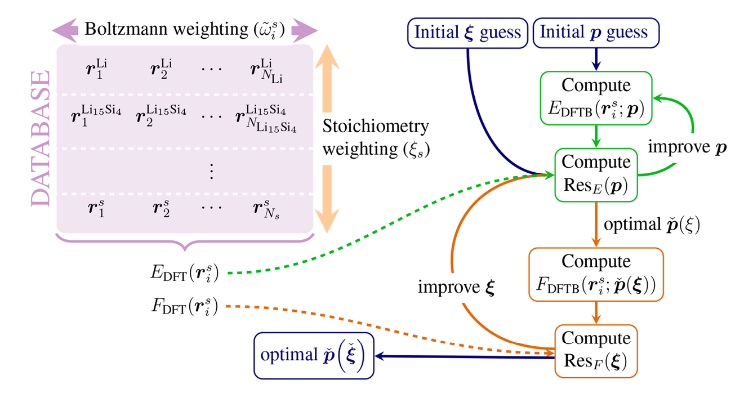
\includegraphics[width=\textwidth]{Silicio/modelo/metodos/diagrama.png}
    \caption{Diagrama de flujo del algoritmo de ajuste. Se realizan dos
    procedimientos de optimización anidados: la minimización de Res$_E$ (ecuación 
    \ref{eq:e_res}) utilizando el código \texttt{TANGO} \cite{tango} (resaltado en
    verde) y la minimización de Res$_F$ (ecuación \ref{eq:fepa}) utilizando un 
    código llamado \texttt{Milonga} (resaltado en naranja). Cada mejora de los pesos
    $\boldsymbol{\xi}$ requiere una minimización completa de Res$_E$ para obtener 
    los parámetros óptimos DFTB asociados $\check{{\bf p}}(\boldsymbol{\xi})$.}
    \label{fig:diagrama}
\end{figure}
